\setcounter{page}{1}
\pagenumbering{arabic}
\chapter{Introduction}\label{Ch1}

\section{Purpose of document}
This report covers the context in which a problem exists and also why it is important to address the problem by providing a short background on devices that measure body temperature, the use thereof, and the working of these devices. Some background information is then used to provide a summary of the problem at hand. A possible solution is then shortly discussed, followed by some high-level objectives that will be pursued in an attempt to solve this problem. Anticipated benefits of the solution, technical requirements, scope of the project, and project deliverables are given to provide more context of this project. 


\section{Background}
Body temperature can be defined as the measure of how well the human body can get rid of and generate heat. Body temperature is needed to sustain and promote human life. The measurement of body temperature plays an important role in our everyday life (especially in the pandemic we find our-self in) since several diseases are characterised by a change in body temperature. Some body temperature measuring devices, such as the clinical thermometer, which is commonly used domestically and in hospitals, must be placed underneath one's tongue or under the armpit. This proves to be unhygienic when these measuring devices are not properly cleaned and can also cause some annoyance for certain people. The need for non-invasive body temperature measuring equipment exists, that can fast and effectively determine body temperature on the move. Mobility will ensure that body temperature readings are always available, anywhere. 
\\
\\
Rotational motions and constant internal vibrations in molecules generate thermal energy or heat. Temperature is therefore a measure of the average thermal energy of molecular motions. Biochemical processes take place inside living cells that contain molecules and are greatly influenced by body temperature \cite{Chen2019}. These biochemical processes are known as metabolism. Humans are homeothermic and body temperature is regulated at about 37°C ± 1°C \cite{Wong2015}. The body needs to maintain its temperature at a certain level to support and stimulate its metabolic activities. Both temperature statuses, hyperthermia (too high) or hypothermia (too low) can alter metabolic activities, cause tissue damage and disturb organic functions. Hence, it is important to examine and monitor body temperature to hunt for signs of diseases that are characterised by a change in body temperature. Body temperature measurements allow doctors and other medical practitioners to analyse the effectiveness of the prescribed treatment. 
\autoref{tab:1} shows both extremes of body temperature and some associated effects at certain temperatures. 

\begin{table}[H]
	\centering
	\caption{\textit{Body temperature effects}\cite{Chen2019}}
	\label{tab:1}
	\begin{tabular}{|c|c|}
		\hline
		\textbf{Temperature} & \textbf{Effect}\\
		\hline
		\hline
		24-28°C & Mostly death.\\
		\hline
		29-33°C & Sleepiness, slow heartbeat, moderate to severe confusion, unresponsive to stimulus.\\
		\hline
		34-35°C & Bluish/Grayness of the skin, intense shivering, numbness and some confusion.\\
		\hline
		36°C & Mild to moderate shivering.\\
		\hline
		37°C & Normal temperature.\\
		\hline
		38-40°C & Dehydration, headache, vomiting and severe sweating.\\
		\hline
		41-42°C & Confusion, fainting, very fast heart rate and high/low blood pressure.\\
		\hline
		43°C & Brain damage, normally death.\\
		\hline
	\end{tabular}
\end{table}
\noindent
Various types of body temperature measuring devices already exist. Some of the most popular domestic-used devices are listed below, each followed by a short description:
\begin{itemize}
	\item Oral Thermometer:\\Most oral thermometers are digital with a housing made out of plastic. This is an invasive device that must be placed under the tongue for a short while allowing it to measure body temperature. The oral thermometer uses thermistor resistance that varies with temperature as sensing element. In many cases, the user will be alerted when the reading is completed. 
	\item Tympanic Thermometer:\\Tympanic Thermometers are minimally invasive since it is placed inside the ear canal to take body temperature readings. This type of device measures the natural emission of infrared thermal radiation from the	tympanic membrane. This digital device has a cone shape designed to fit into an ear. 
	\item Mercury-in-glass/ Alcohol-in-glass Thermometer:\\ This device measures oral, rectal, or armpit body temperature through the thermal expansion of ethanol/mercury. These types of devices are made of glass and the thermal expansion of the ethanol/mercury caused by heat must be noted by the user when taking a reading. 
	\item Infrared Thermometer:\\This is a non-invasive device that measures thermal radiation (infrared) emitted from the forehead and skin to deduce body temperature. The infrared thermometer uses a pyroelectric sensor to measure temperature. Infrared thermometers provides a digital temperature reading and the user could be alerted when this reading is abnormal. 
\end{itemize}
The devices listed have their own advantages and disadvantages. According to \cite{Whelan2020}, oral thermometers are most accurate for children over 3 years of age and adults. The drawback is that, as mentioned earlier, if the device is not cleaned properly it may be unhygienic. The article also mentions that tympanic thermometers provide fast and accurate readings but objects such as earwax and improper positioning may distort results. The Mercury-/Alcohol-in glass thermometers are not digital devices, the user must constantly look at the expansion of the liquid to determine the reading. Infrared thermometers provide quick readings contactless. However, it is believed that these infrared thermometers are not truly as accurate as the rest since external factors, such as direct sunlight and indoor heating, may affect the readings \cite{Whelan2020}.
\\
\\
Throughout this section, mentions of invasive and non-invasive methods were made. These are the two main methods to measure body temperature — by measuring core (deep tissue, invasive) temperature and surface (skin, non-invasive) temperature. Invasive temperature measurements can be taken through the oral cavity, ear canal, and rectum, whilst non-invasive readings are made on the skin surface. In many cases invasive methods cannot be used, such as when someone is unconscious, confused, or sneezing repeatedly, then the oral measurement method is unsuitable. When someone has a middle ear infection or an obstruction in their ear by wax, the ear method is of no use. Non-invasive methods can easily be affected by external factors such as sunlight and indoor heating/cooling. 
\section{Problem Statement}
From the previous section, it is clear that a non-invasive body temperature measuring device is needed that can measure core body temperature, without the readings getting affected by external factors, whilst being comfortable. 

\section{Hypothesis}
A medical wristband that can measure body temperature will be designed and constructed. This allows end-users to wear the device on their wrist, and to see his or her body temperature that is measured and displayed by the wristband. 

\section{Project Objective}
\subsection{Primary Objective}
The primary objective of this project is to design an accurate body temperature measuring device that can be worn as a wristband. The device should measure one's body temperature without the readings getting affected by external factors. The device will predict core body temperature instead of just measuring surface (skin) temperature. 
\\
\\
Since the device will predict core body temperature, a thermal equivalent circuit model will be used to measure core body temperature with a skin-attachable sensor and experimental investigations will be used to further improve this model. Improvements will lead to more accurate readings. A low-level example of a thermal equivalent circuit model can be seen in \autoref{fig:1}.
\begin{figure}[!htbp!]
	\centering
	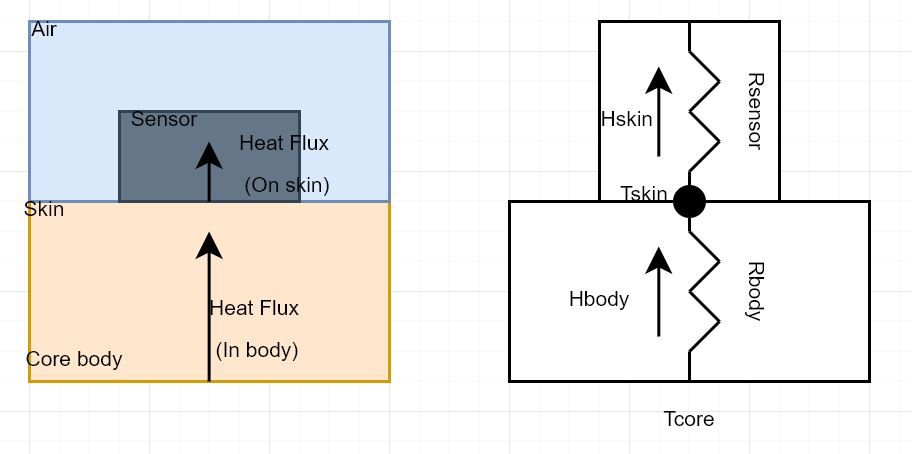
\includegraphics[scale=0.5]{img/Temp_Model}
	\caption{Low level model and thermal equivalent circuit.}
	\label{fig:1}
\end{figure}

\subsection{Secondary Objective}
The device will be able to measure body temperature, this must also be displayed to the user of the wristband. Therefore, the secondary objective is to implement a Human-Machine Interface (HMI). 

\section{Anticipated Benefits of Solution}
The device in the form of a wristband will make the process of measuring body temperature easier and more efficient since the wristband can be comfortably worn throughout the day or night providing continuous readings. These readings are updated by the device on a set interval or on-demand, whilst always displaying the most recent reading. Users will be alerted when the temperature is too high or low so that the necessary steps can be taken right away. This will also be a low-cost, yet reliable build.  

\section{Technical Requirements}\label{1.7}
\subsection{Requirements}
The requirements are listed below:
\begin{enumerate}
	\item Lightweight. The final wristband with the measuring device and the HMI shall be lightweight. This supports the need for a comfortable device. 
	\item Low energy usage. Since the end product will be in the form of a wristband, it will be portable. This means that the measuring device will be battery-powered. Low energy usage shall extend the battery life of the device. 
	\item Cheap. The low-cost aspect of the end product will ensure that the wristband can be widely used by anyone with the need. 
	\item Simple. The device will measure body temperature, show the measured temperature and alert the user when the temperature is outside the set limits.
	\item Accurate. The device shall deliver readings with an accuracy of $\pm$0.5°C to the user of the device. 
	\item The measuring range of the device shall be from 30°C to 40°C, since these temperatures are roughly the limits any living person will achieve.  
	\item The device shall operate in atmospheric temperatures ranging from -5°C to 45°C, making the body temperature measuring device operational in the summer and winter.  
\end{enumerate}

\subsection{Scope Definition}
The scope of the project is to design and implement a body temperature measuring device that can report back a measured reading. Therefore, the sensing element, power supply or battery, and HMI components will not be re-designed, existing components will be used and placed on a Printed Circuit Board (PCB) to make the device small and compact. The wristband itself will not be part of the design, although this can be 3D printed. 

\section{Deliverables}
A device that can measure and display body temperature on the move by placing the device on the wrist will be delivered. This device will be mounted on a wristband that can fit around one's arm at the wrist. Circuit design and PCB layout, together with an enhanced thermal equivalent circuit, or another technique to estimate core body temperature from skin temperature, will also be provided. 

\section{Concluding Remarks}
This section explained the importance of measuring body temperature as it is an indication of a person's physical health status. Some requirements are given, showing what will be incorporated in the final product. The scope definition ensures that all the requirements are reached without doing unnecessary work. 